\documentclass[11pt,a4paper]{report}
\usepackage[textwidth=37em,vmargin=30mm]{geometry}
\usepackage{calc,xunicode,amsmath,amssymb,paralist,enumitem,tabu,booktabs,datetime2,xeCJK,xeCJKfntef,listings}
\usepackage{tocloft,fancyhdr,tcolorbox,xcolor,graphicx,eso-pic,xltxtra,xelatexemoji}

\newcommand{\envyear}[0]{2025}
\newcommand{\envdatestr}[0]{2025-02-05}
\newcommand{\envfinaldir}[0]{webdb/2025/20250205/final}

\usepackage[hidelinks]{hyperref}
\hypersetup{
    colorlinks=false,
    pdfpagemode=FullScreen,
    pdftitle={Web Digest - \envdatestr}
}

\setlength{\cftbeforechapskip}{10pt}
\renewcommand{\cftchapfont}{\rmfamily\bfseries\large\raggedright}
\setlength{\cftbeforesecskip}{2pt}
\renewcommand{\cftsecfont}{\sffamily\small\raggedright}

\setdefaultleftmargin{2em}{2em}{1em}{1em}{1em}{1em}

\usepackage{xeCJK,xeCJKfntef}
\xeCJKsetup{PunctStyle=plain,RubberPunctSkip=false,CJKglue=\strut\hskip 0pt plus 0.1em minus 0.05em,CJKecglue=\strut\hskip 0.22em plus 0.2em}
\XeTeXlinebreaklocale "zh"
\XeTeXlinebreakskip = 0pt


\setmainfont{Brygada 1918}
\setromanfont{Brygada 1918}
\setsansfont{IBM Plex Sans}
\setmonofont{JetBrains Mono NL}
\setCJKmainfont{Noto Serif CJK SC}
\setCJKromanfont{Noto Serif CJK SC}
\setCJKsansfont{Noto Sans CJK SC}
\setCJKmonofont{Noto Sans CJK SC}

\setlength{\parindent}{0pt}
\setlength{\parskip}{8pt}
\linespread{1.15}

\lstset{
	basicstyle=\ttfamily\footnotesize,
	numbersep=5pt,
	backgroundcolor=\color{black!5},
	showspaces=false,
	showstringspaces=false,
	showtabs=false,
	tabsize=2,
	captionpos=b,
	breaklines=true,
	breakatwhitespace=true,
	breakautoindent=true,
	linewidth=\textwidth
}






\newcommand{\coverpic}[2]{
    % argv: itemurl, authorname
    Cover photo by #2~~(\href{#1}{#1})
}
\newcommand{\makeheader}[0]{
    \begin{titlepage}
        % \newgeometry{hmargin=15mm,tmargin=21mm,bmargin=12mm}
        \begin{center}
            
            \rmfamily\scshape
            \fontspec{BaskervilleF}
            \fontspec{Old Standard}
            \fontsize{59pt}{70pt}\selectfont
            WEB\hfill DIGEST
            
            \vfill
            % \vskip 30pt
            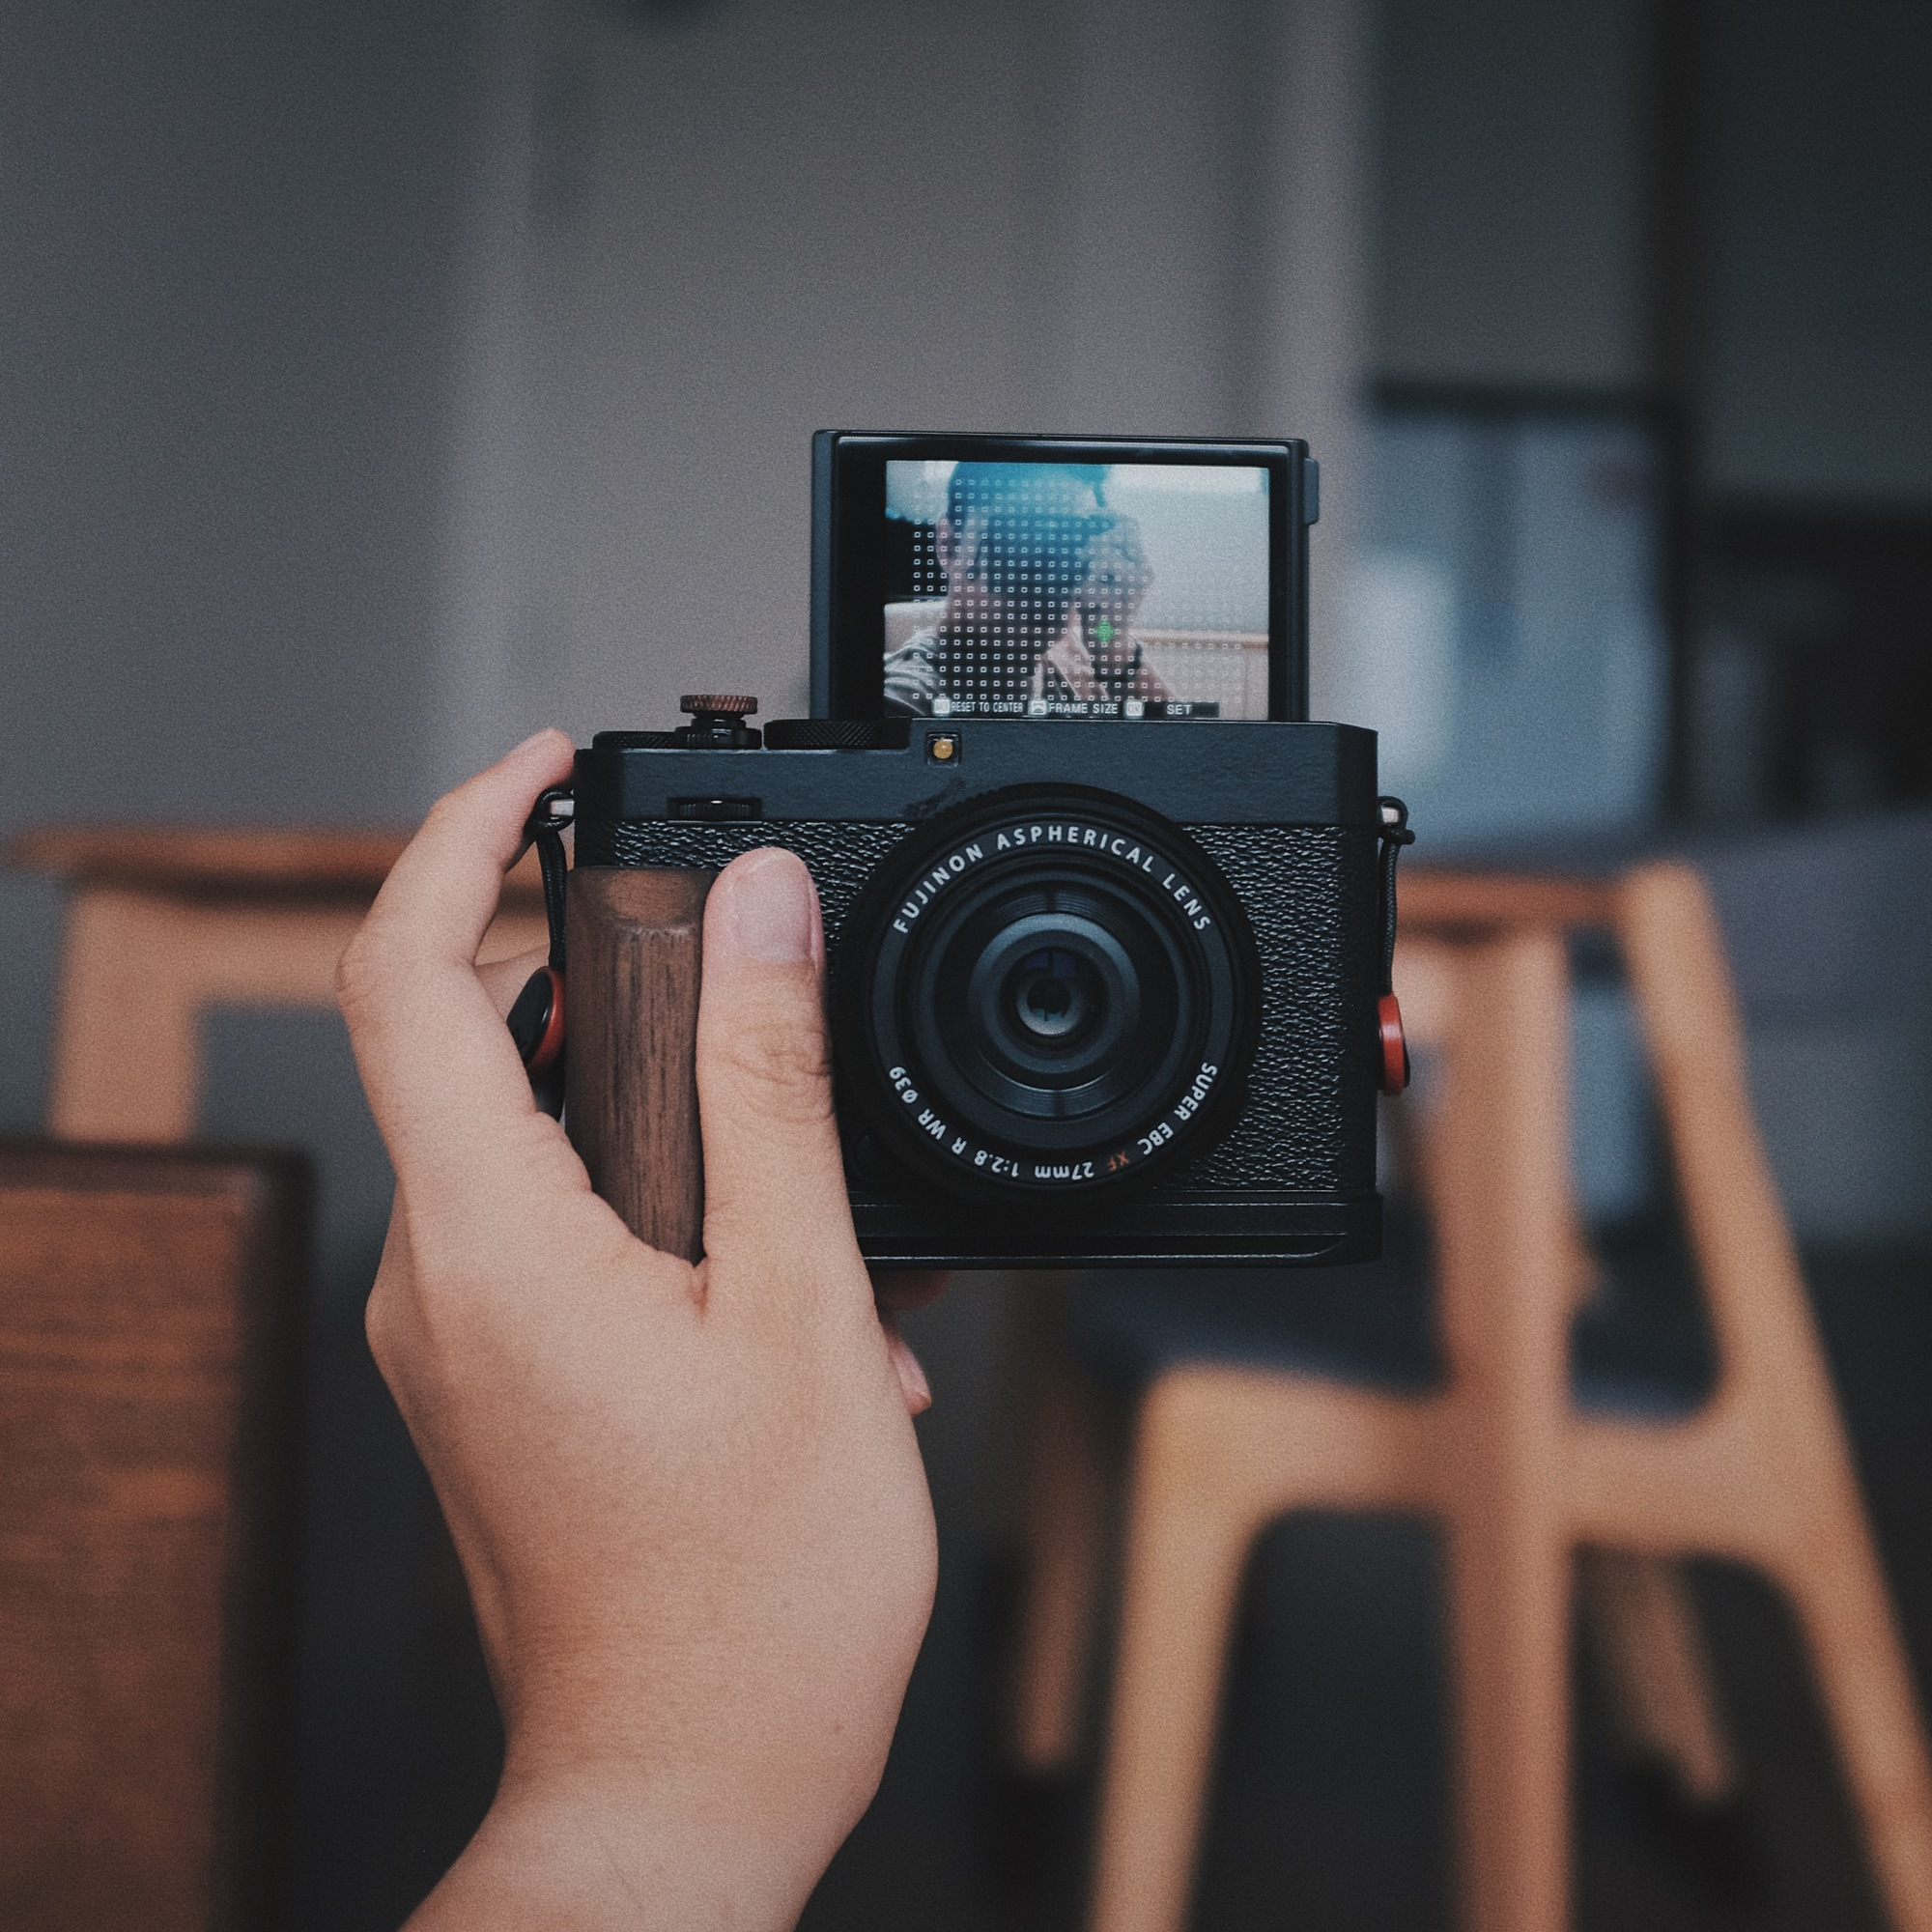
\includegraphics[width=\linewidth]{\envfinaldir/coverpic-prod.jpg}\par
            % \vskip 30pt
            \vfill

            \normalsize\rmfamily\scshape
            \copyright{} The Web Digest Project \hfill\large \envdatestr
        \end{center}
    \end{titlepage}
    % \restoregeometry
}
\newcommand{\simplehref}[1]{%
    \textcolor{blue!80!green}{\href{#1}{#1}}%
}
\renewcommand{\contentsname}{\center\Huge\sffamily\bfseries Contents\par\vskip 20pt}
\newcounter{ipartcounter}
\setcounter{ipartcounter}{0}
\newcommand{\ipart}[1]{
    % \vskip 20pt
    \clearpage
    \stepcounter{ipartcounter}
    \phantomsection
    \addcontentsline{toc}{chapter}{#1}
    % \begin{center}
    %     \Huge
    %     \sffamily\bfseries
    %     #1
    % \end{center}
    % \vskip 20pt plus 7pt
}
\newcounter{ichaptercounter}
\setcounter{ichaptercounter}{0}
\newcommand{\ichapter}[1]{
    % \vskip 20pt
    \clearpage
    \stepcounter{ichaptercounter}
    \phantomsection
    \addcontentsline{toc}{section}{\numberline{\arabic{ichaptercounter}}#1}
    \begin{center}
        \Huge
        \sffamily\bfseries
        #1
    \end{center}
    \vskip 20pt plus 7pt
}
\newcommand{\entrytitlefont}[1]{\subsection*{\raggedright\Large\sffamily\bfseries#1}}
\newcommand{\entryitemGeneric}[2]{
    % argv: title, url
    \parbox{\linewidth}{
        \entrytitlefont{#1}\par\vskip 5pt
        \footnotesize\ttfamily\mdseries
        \simplehref{#2}
    }\vskip 11pt plus 11pt minus 1pt
}
\newcommand{\entryitemGithub}[3]{
    % argv: title, url, desc
    \parbox{\linewidth}{
        \entrytitlefont{#1}\par\vskip 5pt
        \footnotesize\ttfamily\mdseries
        \simplehref{#2}\par\vskip 5pt
        \small\rmfamily\mdseries#3
    }\vskip 11pt plus 11pt minus 1pt
}
\newcommand{\entryitemAp}[3]{
    % argv: title, url, desc
    \parbox{\linewidth}{
        \entrytitlefont{#1}\par\vskip 5pt
        \footnotesize\ttfamily\mdseries
        \simplehref{#2}\par\vskip 5pt
        \small\rmfamily\mdseries#3
    }\vskip 11pt plus 11pt minus 1pt
}
\newcommand{\entryitemHackernews}[3]{
    % argv: title, hnurl, rawurl
    % \parbox{\linewidth}{
    %     \entrytitlefont{#1}\par\vskip 5pt
    %     \footnotesize\ttfamily\mdseries
    %     \simplehref{#3}\par
    %     \textcolor{black!50}{\href{#2}{#2}}
    % }\vskip 11pt plus 11pt minus 1pt
    \begin{minipage}{\linewidth}
            \entrytitlefont{#1}\par\vskip 5pt
            \footnotesize\ttfamily\mdseries
            \simplehref{#3}\par
            \textcolor{black!50}{\href{#2}{#2}}
    \end{minipage}\par\vskip 11pt plus 11pt minus 1pt
}







\begin{document}

\makeheader

\tableofcontents\clearpage




\ipart{Developers}
\ichapter{Hacker News}
\entryitemTwoLinks{Google removes pledge to not use AI for weapons from website}{https://news.ycombinator.com/item?id=42940284}{https://techcrunch.com/2025/02/04/google-removes-pledge-to-not-use-ai-for-weapons-from-website/}

\entryitemTwoLinks{What's Happening Inside the NIH and NSF}{https://news.ycombinator.com/item?id=42940257}{https://www.science.org/content/blog-post/what-s-happening-inside-nih}

\entryitemTwoLinks{Oracle justified its JavaScript trademark with Node.js–now it wants that ignored}{https://news.ycombinator.com/item?id=42939940}{https://deno.com/blog/deno-v-oracle2}

\entryitemTwoLinks{How I use LLMs as a staff engineer}{https://news.ycombinator.com/item?id=42938409}{https://www.seangoedecke.com/how-i-use-llms/}

\entryitemTwoLinks{Google drops pledge not to use AI for weapons or surveillance}{https://news.ycombinator.com/item?id=42938125}{https://www.washingtonpost.com/technology/2025/02/04/google-ai-policies-weapons-harm}

\entryitemTwoLinks{Open Deep Research}{https://news.ycombinator.com/item?id=42937701}{https://github.com/huggingface/smolagents/tree/main/examples/open\_deep\_research}

\entryitemTwoLinks{GitHub reveals how software engineers are purging federal databases}{https://news.ycombinator.com/item?id=42936940}{https://www.404media.co/forbidden-words-github-reveals-how-software-engineers-are-purging-federal-databases/}

\entryitemTwoLinks{How to scale your model: A systems view of LLMs on TPUs}{https://news.ycombinator.com/item?id=42936910}{https://jax-ml.github.io/scaling-book/}

\entryitemTwoLinks{WikiTok}{https://news.ycombinator.com/item?id=42936723}{https://wikitok.vercel.app/}

\entryitemTwoLinks{TikTok's algorithm exhibited pro-Republican bias during 2024 presidential race}{https://news.ycombinator.com/item?id=42936002}{https://www.psypost.org/tiktoks-algorithm-exhibited-pro-republican-bias-during-2024-presidential-race-study-finds/}

\entryitemTwoLinks{How Spotify Killed Lo-Fi Hip Hop}{https://news.ycombinator.com/item?id=42935741}{https://gamechops.substack.com/p/how-spotify-killed-lo-fi-hip-hop}

\entryitemTwoLinks{Roc rewrites the compiler in Zig}{https://news.ycombinator.com/item?id=42935516}{https://gist.github.com/rtfeldman/77fb430ee57b42f5f2ca973a3992532f}

\entryitemTwoLinks{Jujutsu VCS: Introduction and patterns}{https://news.ycombinator.com/item?id=42934427}{https://kubamartin.com/posts/introduction-to-the-jujutsu-vcs/}

\entryitemTwoLinks{Apple Invites}{https://news.ycombinator.com/item?id=42934422}{https://www.apple.com/newsroom/2025/02/introducing-apple-invites-a-new-app-that-brings-people-together/}

\entryitemTwoLinks{Chat is a bad UI pattern for development tools}{https://news.ycombinator.com/item?id=42934190}{https://danieldelaney.net/chat/}

\entryitemTwoLinks{America desperately needs more air traffic controllers}{https://news.ycombinator.com/item?id=42933840}{https://www.cnn.com/2025/02/04/business/air-traffic-controller-shortage/index.html}

\entryitemTwoLinks{100 Or so Books that shaped a Century of Science (1999)}{https://news.ycombinator.com/item?id=42933507}{https://web.mnstate.edu/schwartz/centurylist2.html}

\entryitemTwoLinks{Build a link blog like Simon Willison}{https://news.ycombinator.com/item?id=42933383}{https://xuanwo.io/links/2025/01/link-blog/}

\entryitemTwoLinks{Vanguard's average fee is now 0.07\% after biggest-ever cut}{https://news.ycombinator.com/item?id=42933283}{https://www.bloomberg.com/news/articles/2025-02-03/vanguard-s-average-fee-is-now-just-0-07-after-biggest-ever-cut}

\entryitemTwoLinks{DoppelBot: Replace Your CEO with an LLM}{https://news.ycombinator.com/item?id=42933256}{https://modal.com/docs/examples/slack-finetune}\ichapter{Phoronix}
\entryitemGeneric{\hskip 0pt{}GRUB Continues Working Toward Its Next Release In 2025}{https://www.phoronix.com/news/GRUB-Bootloader-2025}

\entryitemGeneric{\hskip 0pt{}An Early Performance Regression Hitting Highly Threaded Workloads On Linux 6.14-rc1}{https://www.phoronix.com/review/linux-614-early-regression}

\entryitemGeneric{\hskip 0pt{}Firefox 136 Beta Finally Enables Hardware Video Decoding For AMD GPUs On Linux By Default}{https://www.phoronix.com/news/Firefox-136-Beta}

\entryitemGeneric{\hskip 0pt{}FFmpeg Adds AMD AMF Decoder, FSR-Based Upscaling}{https://www.phoronix.com/news/FFmpeg-AMD-AMF-Decoder-FSR}

\entryitemGeneric{\hskip 0pt{}Optimizing The Linux Kernel With PGO Can Yield ~3\% Benefit For HPC Workloads}{https://www.phoronix.com/news/PGO-Optimizations-HPC-3p}

\entryitemGeneric{\hskip 0pt{}Redox OS Makes Progress On Dynamic Linking, New Ports}{https://www.phoronix.com/news/Redox-OS-January-2025}

\entryitemGeneric{\hskip 0pt{}FFmpeg Lands Video Encoding/Decoding Improvements For NVIDIA Blackwell GPUs}{https://www.phoronix.com/news/FFmpeg-Improvements-NV-RTX-50}

\entryitemGeneric{\hskip 0pt{}Ubuntu Infrastructure Woe Continues Making It A Hassle To Run The Latest Upstream Kernel}{https://www.phoronix.com/news/Ubuntu-Mainline-Kernel-Still-No}

\entryitemGeneric{\hskip 0pt{}Linux 6.15 Looks Like It May Try Again With EXECMEM\_ROX Support}{https://www.phoronix.com/news/Linux-EXECMEM\_ROX-Preps-Again}\ichapter{Dribbble}
\entryitemGeneric{\hskip 0pt{}VCC Logo Design Vector Sketches}{https://dribbble.com/shots/25577220-VCC-Logo-Design-Vector-Sketches}

\entryitemGeneric{\hskip 0pt{}S}{https://dribbble.com/shots/25571540-S}

\entryitemGeneric{\hskip 0pt{}Logo and Branding for VCC}{https://dribbble.com/shots/25571598-Logo-and-Branding-for-VCC}

\entryitemGeneric{\hskip 0pt{}Axolotl Mascot}{https://dribbble.com/shots/25572670-Axolotl-Mascot}

\entryitemGeneric{\hskip 0pt{}Finance APP UI Design}{https://dribbble.com/shots/25570740-Finance-APP-UI-Design}

\entryitemGeneric{\hskip 0pt{}Fly Fry}{https://dribbble.com/shots/25573635-Fly-Fry}

\entryitemGeneric{\hskip 0pt{}Cloud Animation Sound Design}{https://dribbble.com/shots/25571319-Cloud-Animation-Sound-Design}

\entryitemGeneric{\hskip 0pt{}Year of the Snake}{https://dribbble.com/shots/25563617-Year-of-the-Snake}

\entryitemGeneric{\hskip 0pt{}Atlantic Pickleball Club}{https://dribbble.com/shots/25558009-Atlantic-Pickleball-Club}

\entryitemGeneric{\hskip 0pt{}Wizard Logo}{https://dribbble.com/shots/25559490-Wizard-Logo}

\entryitemGeneric{\hskip 0pt{}Stellar}{https://dribbble.com/shots/25559656-Stellar}

\entryitemGeneric{\hskip 0pt{}VCC Final Logo Animation}{https://dribbble.com/shots/25557794-VCC-Final-Logo-Animation}

\entryitemGeneric{\hskip 0pt{}Saturday Quiz Time Icons}{https://dribbble.com/shots/25561868-Saturday-Quiz-Time-Icons}

\entryitemGeneric{\hskip 0pt{}Shuttle Robotics}{https://dribbble.com/shots/25557675-Shuttle-Robotics}

\entryitemGeneric{\hskip 0pt{}Real Estate Web Design}{https://dribbble.com/shots/25551949-Real-Estate-Web-Design}

\entryitemGeneric{\hskip 0pt{}Novobet Logo Design - Online Casino Gambling / Betting Platform}{https://dribbble.com/shots/25554663-Novobet-Logo-Design-Online-Casino-Gambling-Betting-Platform}

\entryitemGeneric{\hskip 0pt{}enso homes}{https://dribbble.com/shots/25552493-enso-homes}

\entryitemGeneric{\hskip 0pt{}Stock Trading App}{https://dribbble.com/shots/25554596-Stock-Trading-App}

\entryitemGeneric{\hskip 0pt{}Puzzle Fintech Website Design}{https://dribbble.com/shots/25501121-Puzzle-Fintech-Website-Design}

\entryitemGeneric{\hskip 0pt{}Wardrobe Care Web Design}{https://dribbble.com/shots/25548726-Wardrobe-Care-Web-Design}

\entryitemGeneric{\hskip 0pt{}Columbus Bound®}{https://dribbble.com/shots/25550878-Columbus-Bound}

\entryitemGeneric{\hskip 0pt{}Vista Brand Identity}{https://dribbble.com/shots/25402719-Vista-Brand-Identity}

\entryitemGeneric{\hskip 0pt{}Dave Matthews \& Tim Reynolds 2025 Riviera Maya Branding}{https://dribbble.com/shots/25551625-Dave-Matthews-Tim-Reynolds-2025-Riviera-Maya-Branding}

\entryitemGeneric{\hskip 0pt{}QORE - Logo Design}{https://dribbble.com/shots/25548860-QORE-Logo-Design}


\ipart{Developers~~~~(zh-Hans)}
\ichapter{Solidot}
\entryitemGeneric{\hskip 0pt{}天文学家发现一巨型射电星系}{https://www.solidot.org/story?sid=80466}

\entryitemGeneric{\hskip 0pt{}过去四十年海洋表面变暖速度翻了两番}{https://www.solidot.org/story?sid=80465}

\entryitemGeneric{\hskip 0pt{}Ubuntu 的开发讨论平台将从 IRC 迁移到 Matrix}{https://www.solidot.org/story?sid=80464}

\entryitemGeneric{\hskip 0pt{}Linux 基金会谈论美国 OFAC 制裁和开源项目的应对}{https://www.solidot.org/story?sid=80463}

\entryitemGeneric{\hskip 0pt{}LWN 提供 EPUB 格式的电子书}{https://www.solidot.org/story?sid=80462}

\entryitemGeneric{\hskip 0pt{}苹果开源 Swift Build}{https://www.solidot.org/story?sid=80461}

\entryitemGeneric{\hskip 0pt{}Steam Linux 1 月份额略有下降}{https://www.solidot.org/story?sid=80460}\ichapter{V2EX}
\entryitemGeneric{\hskip 0pt{}[ WATCH] 不带手机去公司, apple watch 能自己连上之前已经连过的 WiFi 吗?}{https://www.v2ex.com/t/1108919}

\entryitemGeneric{\hskip 0pt{}[旅行] 2024 国庆旅游流水账}{https://www.v2ex.com/t/1108918}

\entryitemGeneric{\hskip 0pt{}[问与答] 国内如何买到原生 android TV 电视?}{https://www.v2ex.com/t/1108917}

\entryitemGeneric{\hskip 0pt{}[问与答] Cursor tab 的 prompt 是什么?}{https://www.v2ex.com/t/1108916}

\entryitemGeneric{\hskip 0pt{}[问与答] 有懂直流无刷电机的朋友,请教几个问题}{https://www.v2ex.com/t/1108915}

\entryitemGeneric{\hskip 0pt{}[问与答] 求推荐 chrome 有没有下载加速插件?}{https://www.v2ex.com/t/1108914}

\entryitemGeneric{\hskip 0pt{}[Twitter] 什么时候开始国区 app store 可以直接下载 X 了?}{https://www.v2ex.com/t/1108913}

\entryitemGeneric{\hskip 0pt{}[程序员] XXL-CACHE v1.1.0 | 多级缓存框架}{https://www.v2ex.com/t/1108912}

\entryitemGeneric{\hskip 0pt{}[分享发现] 刚出炉的 ! 2025 年香港银行开户攻略,中银万事达、汇丰、众安、蓝狮子、实体卡下卡成功}{https://www.v2ex.com/t/1108911}

\entryitemGeneric{\hskip 0pt{}[OpenWrt] 有老哥能协助装下 N1 openwrt 么?请杯奶茶}{https://www.v2ex.com/t/1108910}

\entryitemGeneric{\hskip 0pt{}[分享创造] 浏览器助手 Lokica v1.3.0 发布了~新增滑词翻译, newtab 和悬浮球可以在选项里开启关闭啦}{https://www.v2ex.com/t/1108909}

\entryitemGeneric{\hskip 0pt{}[问与答] @v2exPush 这个 V2 的 tg 推送频道主请出来}{https://www.v2ex.com/t/1108908}

\entryitemGeneric{\hskip 0pt{}[分享创造] 写了 10 年的音乐播放器,第 11 年有了 AI 加持!}{https://www.v2ex.com/t/1108907}

\entryitemGeneric{\hskip 0pt{}[程序员] 假设 deepseek 一直被攻击,是不是服务会一直繁忙?}{https://www.v2ex.com/t/1108905}

\entryitemGeneric{\hskip 0pt{}[Android] 给老婆买手机,求推荐}{https://www.v2ex.com/t/1108904}

\entryitemGeneric{\hskip 0pt{}[宽带症候群] 联通也开始搞 ip 段限速了吗}{https://www.v2ex.com/t/1108903}

\entryitemGeneric{\hskip 0pt{}[问与答] 如何只同步 A 目录下新加入的文件到 B 目录下?}{https://www.v2ex.com/t/1108902}

\entryitemGeneric{\hskip 0pt{}[Apple] iCloud 空间不够全量同步,我希望它能尽量同步,但同步开关打不开了,有办法吗?}{https://www.v2ex.com/t/1108901}

\entryitemGeneric{\hskip 0pt{}[Android] 怎样绕过得物 App 的 Root 检测?}{https://www.v2ex.com/t/1108900}

\entryitemGeneric{\hskip 0pt{}[电影] 哪吒看完了,给不了 6 分,就喷这一点}{https://www.v2ex.com/t/1108899}

\entryitemGeneric{\hskip 0pt{}[程序员] Hyper-V GPU 分区玩游戏 vmmem 进程的内存占用很不正常,我给虚拟机分 32GB 运行内存, vmmem 进程的 Commit Size 经常跑到 130GB 以上,然后把虚拟内存占满了,导致主机黑屏}{https://www.v2ex.com/t/1108898}

\entryitemGeneric{\hskip 0pt{}[问与答] DeepSeek App 的后端服务又又又崩了(2025-02-04)?}{https://www.v2ex.com/t/1108897}

\entryitemGeneric{\hskip 0pt{}[微信] 有没有多台 PC 设备同时使用微信客户端的方法?}{https://www.v2ex.com/t/1108894}

\entryitemGeneric{\hskip 0pt{}[问与答] Mac 上蓝牙键盘和触摸板间歇性间断,排查思路?}{https://www.v2ex.com/t/1108892}

\entryitemGeneric{\hskip 0pt{}[问与答] 求个最新的 N1 旁路由固件… 找了好多都不太靠谱}{https://www.v2ex.com/t/1108891}

\entryitemGeneric{\hskip 0pt{}[程序员] 请问一下大伙儿, 现在``最快的'' DeepSeek API 是哪家?}{https://www.v2ex.com/t/1108888}

\entryitemGeneric{\hskip 0pt{}[全球工单系统] 豆瓣又挂了?}{https://www.v2ex.com/t/1108887}

\entryitemGeneric{\hskip 0pt{}[路由器] 求大佬推荐路由器或者软路由,要求 Xray+Xhttp+reality 能跑满 500m 的}{https://www.v2ex.com/t/1108886}

\entryitemGeneric{\hskip 0pt{}[问与答] 请教,哪家云厂商的 DeepSeekR1 是自己部署的?}{https://www.v2ex.com/t/1108884}

\entryitemGeneric{\hskip 0pt{}[分享发现] 7 块钱注册 Claude,感觉亏了}{https://www.v2ex.com/t/1108883}

\entryitemGeneric{\hskip 0pt{}[问与答] 我的项目是开源项目二次开发的,今天突然提示这个}{https://www.v2ex.com/t/1108880}

\entryitemGeneric{\hskip 0pt{}[宽带症候群] 湖南电信融合宽带 1000 兆每月 199 包月,换套餐想保留公网 IP 怎么办?}{https://www.v2ex.com/t/1108879}

\entryitemGeneric{\hskip 0pt{}[开源软件] Obsidian 下有没有可以双向同步 Memos 的插件?}{https://www.v2ex.com/t/1108878}

\entryitemGeneric{\hskip 0pt{}[问与答] 1Password 7 不能打开了}{https://www.v2ex.com/t/1108877}

\entryitemGeneric{\hskip 0pt{}[职场话题] 从其他行业转行到开发的,你们现在怎样了,后悔了吗?}{https://www.v2ex.com/t/1108876}

\entryitemGeneric{\hskip 0pt{}[宽带症候群] IPv6 大数据包传输测试超时}{https://www.v2ex.com/t/1108875}

\entryitemGeneric{\hskip 0pt{}[酷工作] [远程 Web3 交易所] - 风控策略专员}{https://www.v2ex.com/t/1108874}

\entryitemGeneric{\hskip 0pt{}[程序员] 访问 V2EX 的问题}{https://www.v2ex.com/t/1108873}

\entryitemGeneric{\hskip 0pt{}[问与答] 新买的电脑可以做哪些设置?}{https://www.v2ex.com/t/1108872}

\entryitemGeneric{\hskip 0pt{}[问与答] MAC QQ 老版本哪一个现在可以正常运行?}{https://www.v2ex.com/t/1108870}

\entryitemGeneric{\hskip 0pt{}[问与答] 买了个欧版 S25U,我看 imei 是质保已经在 2 周前被激活?}{https://www.v2ex.com/t/1108867}

\entryitemGeneric{\hskip 0pt{}[推广] 25 年元旦新西兰激活 skinny 电话卡¥78 包邮}{https://www.v2ex.com/t/1108866}

\entryitemGeneric{\hskip 0pt{}[随想] 过年回家,没网,不探亲,没人认识,麻了}{https://www.v2ex.com/t/1108864}

\entryitemGeneric{\hskip 0pt{}[宽带症候群] 上海移动是不是识别 wg 协议,限速了?(非出国)}{https://www.v2ex.com/t/1108861}

\entryitemGeneric{\hskip 0pt{}[Notion] notion 有相同用户经历的吗?}{https://www.v2ex.com/t/1108860}

\entryitemGeneric{\hskip 0pt{}[问与答] 有台湾的朋友认识 陈晓舟​黄兰英​ 夫妻吗?}{https://www.v2ex.com/t/1108859}

\entryitemGeneric{\hskip 0pt{}[Steam] steam deck 换了下硬盘,电源芯片烧了,苏州上海有没有介绍的维修店?}{https://www.v2ex.com/t/1108858}

\entryitemGeneric{\hskip 0pt{}[问与答] 准备用手机 App 云听会员听广播,麻烦问一下坛友有云听会员不用要出的吗?}{https://www.v2ex.com/t/1108856}

\entryitemGeneric{\hskip 0pt{}[分享发现] 疑似 github 学生包不能使用大陆邮箱?}{https://www.v2ex.com/t/1108855}

\entryitemGeneric{\hskip 0pt{}[程序员] deepseek 识别图像的疑惑}{https://www.v2ex.com/t/1108854}


\ipart{Generic News}







\clearpage
\leavevmode\vfill
\footnotesize

Copyright \copyright{} 2023-2025 Neruthes and other contributors.

This document is published with CC BY-NC-ND 4.0 license.

The entries listed in this newsletter may be copyrighted by their respective creators.

This newsletter is generated by the Web Digest project.

The newsletters are also delivered via Telegram channel \CJKunderline{\href{https://t.me/webdigestchannel}{https://t.me/webdigestchannel}}.\\
RSS feed is available at \CJKunderline{\href{https://webdigest.pages.dev/rss.xml}{https://webdigest.pages.dev/rss.xml}}.

This newsletter is available in PDF at
\CJKunderline{\href{https://webdigest.pages.dev/}{https://webdigest.pages.dev/}}.

The source code being used to generate this newsletter is available at\\
\CJKunderline{\href{https://github.com/neruthes/webdigest}{https://github.com/neruthes/webdigest}}.

This newsletter is also available in
\CJKunderline{\href{http://webdigest.pages.dev/readhtml/\envyear/WebDigest-20250205.html}{HTML}} and
\CJKunderline{\href{https://github.com/neruthes/webdigest/blob/master/markdown/\envyear/WebDigest-20250205.md}{Markdown}}.


\coverpic{https://unsplash.com/photos/the-sun-is-setting-over-the-ocean-with-waves-7CI8rwe8g4U}{Gustavo Zambelli}


\end{document}
